% !TeX spellcheck = en_GB

\section{Algorithms}\label{algorithms}

\subsection{Help Data Structure Pyramid and Others}

\noindent Define $[i,\ j]$: \\
$[i,\ j] := \{i,\ i+1,..., j-1,\ j\} \subseteq \mathbb{N}_{\geq 0}$.\\

\noindent Define $Pyramid$:\\
$Pyramid :=\{ cell_{i,j}\ |\ i \in \mathbb{N}_{\geq 0},\  j \in [0,\ j_{max}-i],\ i_{max} = j_{max} = |word|-1\}$.\\
$cell_{i,j} = \{c\ |\ c \subseteq V\}$.\\
$EmptyPyramid \Leftrightarrow \forall i\ \forall j\ cell_{i,j}=\emptyset$.\\
Regarding one $cell_{i,j}$: $cell_{i,j} = cellDown$, $cell_{i-1,j} = cellUpperLeft$ and $cell_{i-1,j+1} = cellUpperRight$  \\

\begin{figure}[h]
	\centering
	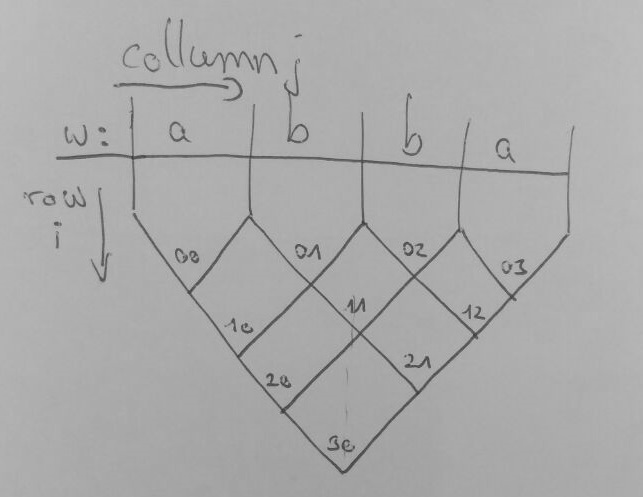
\includegraphics[width=0.7\textwidth]{abb/DataStructurePyramid}
\end{figure}
\pagebreak
\begin{center}
	\resizebox{0.9\linewidth}{!}{
		\begin{tikzpicture}[baseline]
		% Outer hull
		\coordinate (top) at (3,-3);
		\draw [thick, orange] (top) circle [radius=0.1];
		\draw[help lines] (-1,1) grid (6,-3);
		\draw [brown, ultra thick] (0,0) circle [radius=0.1];
		%\coordinate (top) at (2.5,-2.5);
		\draw [->, thick] (-0.5,1) -- (0.5,1);
		\node [above] at (0, 1) {i};
		\draw [->, thick] (-0.5,1) -- (-0.5,-0.0);
		\node [left] at (-0.5,0.5) {j};
		
		\draw [thick, red] (2,-1) circle [radius=0.1];
		\draw [thick, black] (2,-0.5) circle [radius=0.01];
		\coordinate (center) at (2, -0.5);
		\node [left] at (center) {\fontsize{5}{12}\selectfont{A1}};
		\node [above] at (center) {\fontsize{5}{12}\selectfont{B2}};
		\node [right] at (center) {\fontsize{5}{12}\selectfont{C3}};
		\node [below] at (center) {\fontsize{5}{12}\selectfont{D4}};
		\node [] at (center) {\fontsize{5}{12}\selectfont{E5}};
		
		\foreach \i in {0,...,6} {
			\coordinate (\i) at (\i,0);
			\draw [thick] (\i,0) circle [radius=0.2];
		}
		
		% Draw the left and right line of the pyramid pointing downwards
		\draw (0) -- (top) -- (6);
		
		% Grid lines direction top-left to down-right
		\foreach \coord/\i in {right1/.17,right2/.34,right3/.5,right4/.68,right5/.85} {
			\coordinate (\coord) at ($(top)!\i!(6)$);
			\draw [thick, blue] (\i,0) circle [radius=0.1];
		}
		\foreach \i/\coord in {1/right1,2/right2,3/right3,4/right4,5/right5}{
			\draw (\i) -- (\coord);
			\draw [thick, blue] (\i,0) circle [radius=0.1];
		}
		
		% Grid lines direction top-right to down-left
		\foreach \coord/\i in {left1/.17,left2/.34,left3/.5,left4/.68,left5/.85} {
			\coordinate (\coord) at ($(0)!\i!(top)$);
			\draw [thick, red] (\i,0) circle [radius=0.05];
		}
		\foreach \i/\coord in {1/left1,2/left2,3/left3,4/left4,5/left5} {
			\draw (\i) -- (\coord);
			\draw [thick, red] (\i,0) circle [radius=0.05];
		}
		
		% Small lines at the top
		\foreach \i in {0,...,6} {
			\draw (\i) -- ($(\i)+(0,.5)$);
		}
		
		% The string
		\foreach \i/\j/\k in {0/1/b,1/2/b,2/3/a,3/4/c,4/5/b,5/6/c} {
			\node[yshift=.7cm] at ($(\i)!.5!(\j)$) {$\k$};
		}
		\end{tikzpicture}
	}
\end{center}

\begin{center}
	\resizebox{.6\linewidth}{!}{
		\begin{tikzpicture}[-,>=stealth',shorten >=1pt,auto,node distance=2cm,
		semithick]%,initial text={}]
		\tikzstyle{every state}=[fill=white,draw=black,text=black]
		
		\node     (I)            {$S1$};
		\node				(I') [below left of=I] {};
		\node (B) [left of=I']  {$A1$};
		\node (B1) [below of=B] {$c$};
		\node (C) [below right  of=I]       {$B6$};
		\node (D) [below right of=C]  {$B7$};
		\node (D2) [below left of=C]  {$C4$};
		\node (E) [below right of=D]  {$B8$};
		\node (F1) [below of=E]  {$b$};
		\node (E1) [below of=D]  {$C7$};
		\node (E3) [below of=D2]  {$C5$};
		\node (E2) [below left of=D2]  {$A2$};
		\node (F) [below  of=E1]  {$c$};
		\node (F3) [below of=E3]  {$A5$};
		\node (G1) [below  of=F3]  {$a$};
		\node (F2) [below right of=E3]  {$C6$};
		\node (G2) [below  of=F2]  {$c$};
		\node (H1) [below of=E2]  {$A3$};
		\node (H2) [below left of=E2]  {$B2$};
		\node (H3) [below left of=H2]  {$b$};
		\node (J1) [below of=H1]  {$A4$};
		\node (K1) [below of=J1]  {$a$};
		\node (J2) [below left of=H1]  {$B3$};
		\node (K3) [below of=J2]  {$b$};
		
		\path 
		(I) edge   node {$ $}   (B)
		(I) edge   node {$ $}   (C)
		(B) edge   node {$ $}   (B1)
		(C) edge   node {$ $}   (D)
		(D) edge   node {$ $}   (E)
		(C) edge   node {$ $}   (D2)
		(D2) edge   node {$ $}   (E3)
		(D) edge   node {$ $}   (E1)
		(D2) edge   node {$ $}   (E2)
		(E1) edge   node {$ $}   (F)
		(E) edge   node {$ $}   (F1)
		(E3) edge   node {$ $}   (F3)
		(E3) edge   node {$ $}   (F2)
		(F2) edge   node {$ $}   (G2)
		(F3) edge   node {$ $}   (G1)
		(E2) edge   node {$ $}   (H2)
		(E2) edge   node {$ $}   (H1)
		(H2) edge   node {$ $}   (H3)
		(H1) edge   node {$ $}   (J2)
		(H1) edge   node {$ $}   (J1)
		(J1) edge   node {$ $}   (K1)
		(J2) edge   node {$ $}   (K3)
		;
		
		\end{tikzpicture}
	}
	
\end{center}

\pagebreak
\subsection{Exam Exercise Generating Algorithms}

\pagebreak

\subsubsection{Algorithm: AlgorithmName}
\noindent Things like the $G=(V,\Sigma , S, P)$ can be assumed as known.\\
$P = P \cup \{distribute\ \{\sigma\ |\ \sigma \in w \}\ uniform\ randomly\ over\ \{v\ |\ v \in V \} \}$ which equals the $distributeRhse$ module.\\
\noindent Bias is only allowed top vs down regarding the pyramid. No left or right bias intended yet.\\
\circled{A}, \circled{B}, ... represent exchangeable algorithm modules. 

\paragraph{Basic Idea}

\paragraph{Tweak Idea 1 for Algorithm}

\paragraph{Tweak Idea 2 for Algorithm}

\paragraph{Finished Algorithm}



\pagebreak

\subsubsection{Algorithm: GeneratorGrammarDiceRollOnly}
\noindent Very naive way of generating grammars. This is intended to be the starting point for our algorithms we find. Each found algorithm must have a higher score than this algorithm or otherwise it would be worse than simple dice rolling and then removing the useless productions.\\

\noindent
\frame{
	\begin{algorithm}[H] %or another one check
		\caption{GeneratorGrammarDiceRollOnly}
		\label{GeneratorGrammarDiceRollOnly}
		\SetAlgoLined
		\KwIn{ $Word\ w \in \Sigma^{*}$ }
		\KwOut{$ P \subseteq V \times (V^{2} \cup \Sigma)$}
		$P = \{distribute\ \sigma \in \Sigma\ over\ V \} $; \circled{A} \\
		$P = P \cup \{distribute\ vc \in V^2\ over\ V \}$; \circled{B} \\
		$P = P \setminus \{p\ |\ p \subseteq P,\ vc\ is\ right\ in\ p,\ \forall i\ \forall j\ vc \notin cell_{i,j}\ of\ the\ pyramid \}\label{useless} $\;
		\Return $P$\;
		\footnotetext{
			\noindent Line \ref{useless}: Removes all useless production.
		}
	\end{algorithm}
}
Does the output $P \subseteq V \times (V^{2} \cup \Sigma)$ imply that $G$ is in CNF? CNF does only have useful variables [TI script Def. 8.3 page 210] vs. $P \subseteq V \times (V^{2} \cup \Sigma)$\\
%\frame{
%	\begin{algorithm}[H] %or another one check
%		\caption{GeneratorGrammarDiceRollOnly}
%		\label{GeneratorGrammarDiceRollOnly}
%		\SetAlgoLined
%		\KwIn{ $Word\ w \in \Sigma^{*},\ P \subseteq V \times (V^{2} \cup \%Sigma) = \emptyset,\ $ }
%		\KwOut{$Grammar\ G\ in\ CNF$}
%		
%		$P = P \cup \{distribute\ \{\sigma\ |\ \sigma \in w \}\ over\ \{v\ |\ v% \in V \} \} $\;
%		$P = P \cup \{distribute\ \{vc\ |\ vc \in V^2 \}\ $$over\ \{v\ |\ v \in V \} \} $\;
%		$P = P \setminus \{p\ |\ p \subseteq P,\ vc\ is\ right\ in\ p,\ \forall i\ \forall j\ vc \notin cell_{i,j}\ of\ the\ pyramid \} $\;
%		\Return $G$\;
%	\end{algorithm}
%}
\noindent
\frame{
	\begin{algorithm}[H] %or another one check
		\caption{GeneratorGrammarDiceRollOnlyBias}
		\label{GeneratorGrammarDiceRollOnlyBias}
		\SetAlgoLined
		\KwIn{ $Word\ w \in \Sigma^{*},\ P \subseteq V \times (V^{2} \cup \Sigma) = \emptyset,\ $ }
		\KwOut{$Grammar\ G\ in\ CNF$}
		
		NOT FINISHED, MAYBE LATER.\\		
		$pick\ uniform\ randomly\  \{v\ |\ v \in V\} with...\ $\;
		$...$\;
		$P = P \cup \{distribute\ \{\sigma\ |\ \sigma \in w \}\ over\ \{v\ |\ v \in V \} \} $\;
		$P = P \cup \{distribute\ \{vc\ |\ vc \in V^2 \}\ $$over\ \{v\ |\ v \in V \} \} $\;
		$P = P \setminus \{p\ |\ p \subseteq P,\ vc\ is\ right\ in\ p,\ \forall i\ \forall j\ vc \notin cell_{i,j}\ of\ the\ pyramid \} $\;
		\Return $G$\;
	\end{algorithm}
}

\pagebreak
\subsubsection{Algorithm: BottomUp GeneratorGrammarDiceRollMartens}
\noindent
\frame{
	\begin{algorithm}[H] %or another one check
		\caption{GeneratorGrammarDiceRollMartens}
		\label{GeneratorGrammarDiceRollMartens}
		\SetAlgoLined
		\KwIn{ $Word\ w \in \Sigma^{*}$ }
		\KwOut{$P \subseteq V \times (V^{2} \cup \Sigma)$}
		
		$P = \{distribute\ \sigma \in \Sigma\ over\ V \} $; \circled{A} \\
		$pyramid = CYK(G,\ w)$\label{stepii}\;
		\For{$i:=1\ \textbf{to}\ i_{max}$}{
			$J \subseteq \mathbb{N}$\;
			$cellSet \subseteq V^2$\;
			\While{$|J| < j_{max}-i$}{
				$choose\ one\ j \notin J\ uniform\ randomly\ in\ [0, j_{max}-i] $ \label{chooseJ} \;
				$J = J \cup j$\;
				$cellSet = calculateSubsetForCell(pyramid,\ i,\ j)$\;
				$P = P \cup \{distribute\ vc \in cellSet\ over\ V \}$;  \circled{B} \\
				$pyramid = CYK(G,\ w)$\;	
				$evaluate\ stopping\ criteria\ regarding\ the\ pyramid$;  \circled{C} \\
				\If{$stopping\ criteria = true$}{
					\Return $P$\;
				}
			}
		}
		\Return $P$\;
		\footnotetext{
			\noindent Line \ref{stepii}: Fills the i=0 row of the pyramid.
			
			\noindent Line \ref{chooseJ}: Instead of going from left to right, choose $j$ uniform randomly with the restrictions that one cell is only visited one time.
			
			\noindent Note: Maybe modify algorithm to also work with the threshold.
		}
	\end{algorithm}
}

\noindent
\frame{
	\begin{algorithm}[H] %or another one check
		\caption{GeneratorGrammarDiceRollMartens2}
		\label{GeneratorGrammarDiceRollMartens2}
		\SetAlgoLined
		\KwIn{ $Word\ w \in \Sigma^{*}$ }
		\KwOut{$P \subseteq V \times (V^{2} \cup \Sigma)$}
		$P = \{distribute\ \sigma \in \Sigma\ over\ V \} $; \circled{A}  \\
		$pyramid = CYK(G,\ word)$ \label{stepii}\;
		\For{$i:=1\ \textbf{to}\ i_{max}$}{
			%$choose\ j\ uniform\ randomly\ in\ [0,\ j_{max}-i]  $\;
			\For{$j:=0\ \textbf{to}\ j_{max}-i$}{
				$rowSet = rowSet \cup \{(XY,i)\ |\ X,Y \in V,\ $ $XY \in calculateSubsetForCell(Pyramid,\ i,\ j) \}$\label{rowSet}\;
			}
			\While{$threshold_i = false $}{
				$choose\ one\ vc \in rowSet\ with\ priority,\ depending\ on\ i,\ $ $ uniform\ randomly$;\label{chooseVc} \circled{D}  \\
				$P = P \cup \{distribute\ vc \in rowSet\ over\ V\} $; \circled{B}  \\
				$pyramid = CYK(G,\ w)$\;
				$evaluate\ and\ update\ threshold_i,\ regarding\ line\ i$\label{threshold}\;
				$evaluate\ stopping\ criteria,\ regarding\ the\ pyramid$; \circled{C} \\
				\If{$stopping\ criteria = true$}{
					\Return $P$\;
				}	
			}
		}
		\Return $P$\;
		\footnotetext{
			\noindent Line \ref{stepii}: Fills the i=0 row of the pyramid.
			
			\noindent Line \ref{rowSet}: $(AB,1), (AB,2), (BC,3) ... \in sub$ $\rightarrow$ multiple occurrences of $AB$ are allowed. This considers "more important" compound variables. 
			
			\noindent Line \ref{chooseVc}: One vc can be chosen several times.
			
			\noindent Note Line \ref{chooseVc}: Priority mechanism: In line $i+1$ the $k = \{(A,l)\ |\ (A,l) \in sub,\ l=i  \}$ are preferred over the\\ $m = \{(A,n)\ |\ (A,n) \in sub,\ n < i  \}$. In what way are they preferred? Using some kind of factor to weight the $i$ of $(A,i)$.
			
			\noindent Note Line \ref{threshold}: Threshold, Linear or log function $f(i)$?
		}
	\end{algorithm}
}
\pagebreak 
\subsubsection{Algorithm: Idea 1, TopDown From node to leaves}

\noindent
\frame{
	\begin{algorithm}[H] %or another one check
		\caption{Idea1}
		\label{Idea1}
		\SetAlgoLined
		\KwIn{ $Word\ w \in \Sigma^{*},\ i,j \in \mathbb{N},\ \forall j\ cell_{0,j} \neq \emptyset $ }
		\KwOut{$P \subseteq V \times (V^{2} \cup \Sigma)\ or\ cell_{i,j} \subseteq V$}
		\If{$i=0$}{
			\Return $cell_{i,j}$\;
		}
		$choose\ one\ m\ uniform\ randomly\ in\ [j,\ j+i-1]$\label{max}\label{boundsM}\;
		$A = Idea1(w,\ P,\ m,\ j)$\label{cells}\;
		$B = Idea1(w,\ P,\ (i-m),\ (m+j+1))$\;
		$VC = uniform\ random\ subset\ [of\ size\ ?x?]\ from\ \{vc\ |\ v \in A\ \wedge\ c \in B\}$\;
		$P = P \cup \{distribute\ vc \in VC\ over\ V \} $; \circled{A}  \\
		\Return $P$\;
		\footnotetext{
			\noindent Line \ref{boundsM}: $m_{min}=j$ equals the shift in the word and $m_{max}=j+i-1$ [height of the triangle $h(i)$] that equals exactly the size of the following inspected sub string.
			
			\noindent Line \ref{cells} $\longrightarrow\ new\ cells:\ cell_{m, j}\ and\ cell_{i-m, m+j+1}\ See\ Alg.\ subSetCalc\ with\ k \in [i-1;0]\ [Y \in V_{k,j},\ Z \in V_{i-k-1,k+j+1}] $
		}
	\end{algorithm}
}
Algorithm \ref{Idea1} uniform randomly generates a predefined structure of the derivation tree. You always update the pyramid after adding one production to the grammar. Now there are two options to fill the parse table:
\begin{enumerate}
	\item Bottom Up: The parse table is filled relatively evenly. All information regarding the upper cells are available and can be used. Similar to the CYK Algorithm approach.
	\item Top Down: The parse table is filled quiet unevenly. You don't have all information available. Think about adding a production for the node cell: You can add a production so that its producing cells fill the node cell, but you don't know what actually would be the best to fill in these producing cells because they themselves aren't looked at yet. This problem is kept until the last depth of the recursion, where the cells in row $i=0$ are taken into account. Only starting there you know what variables actually produce the terminals.\\
	Maybe solution: For the Top Down approach, don't assume that the terminals are already distributed over the V. Distribute the terminals over the variables in an ideal way that fits your already generated productions best.
\end{enumerate}
The stopping criteria would be, that each marked $cell_{i,j} \neq \emptyset$ and it must be possible to get from $cell_{m, j}$ and $cell_{i-m, m+j+1}$ to $cell_{i,j}$ through applying one of the production rules.

\pagebreak

\subsubsection{Algorithm: Idea 2, How often cells are used for subset calculations}

\pagebreak

\subsubsection{Tweaking Sub Procedures in more detail}
Maybe don't keep this so that the Algorithms can be read without flipping pages.\\

\noindent
\frame{
	\begin{algorithm}[H] %or another one check
		\caption{distributeRhse2}
		\label{distributeRhse2}
		\SetAlgoLined
		\KwIn{ $Rhse \subseteq\ (V^{2} \cup \Sigma),\ i \in  \mathbb{N},\ j \in  \mathbb{N}$}
		\KwOut{$Grammar\ G\ in\ CNF\ with\ uniform\ randomly\ distributed\ Rhse's.$}
		$choose\ n\ uniform\ randomly\ in\ [i, j]$\;
		$choose\ V_{add} := uniform\ random\ subset\ of\ size\ n\ from\ V$\;
		$P = P \cup \{ "v \longrightarrow rhse"\ |\ v \in V_{add},\ rhse \in Rhse \} $\;	
		
		\Return $G$;
	\end{algorithm}
}
Algorithm \ref{distributeRhse2} isn't needed anymore for the descriptions of the basic idea of the algorithm. It will be a module later on while tweaking the algorithms.
\\
\\
\frame{
	\begin{algorithm}[H] %or another one check
		\caption{calculateSubsetForCell}
		\label{calculateSubsetForCell}
		\SetAlgoLined
		\KwIn{$cell_ {i,j} \in pyramid $}
		\KwOut{$V_{i,j} \subseteq V^2$}
		$V_{i,j} = \emptyset $\;
		\For{$k:=i-1 \to 0$}{
			$V_{i,j} = V_{i,j} \cup \{X\ |\ X\longrightarrow YZ,\ Y \in V_{k,j},\ Z \in V_{i-k-1,k+j+1} \}$\;
		}
		
		\Return $V_{i,j}$\;
	\end{algorithm}
}
Algorithm \ref{calculateSubsetForCell} describes the magic of the CKY-algorithm. It shows what cells are taken into account while filling one cell of the parse table.

\pagebreak

\subsection{Criteria Checking Procedures}
\noindent Description of the checks here. \\
\noindent All test of the GrammarValidityChecker class are based on the simple setV matrix. \\

\noindent  isValid = isWordProducible \&\& isExamConstraints \&\& isGrammarRestrictions\\

\noindent  isWordProducible = CYK.algorithmAdvanced()\\

\noindent  isExamConstraints = isRightCellCombinationsForced \&\& isMaxSumOfProductionsCount \&\& isMaxSumOfVarsInPyramidCount \&\& countRightCellCombinationsForced \\

\noindent isGrammarRestrictions = isSizeOfWordCount \&\& isMaxNumberOfVarsPerCellCount \\
\\
\\
\noindent 
\frame{
	\begin{algorithm}[H] %or another one check
		\caption{checkForceCombinationPerCell}
		\label{checkRightCellPerCombination}
		\SetAlgoLined
		\KwIn{$ cell_{i,j}\subseteq V,\ cell_{i-1,j}\subseteq V,\ cell_{i-1,j+1} \subseteq V,\ P \subseteq V \times (V^{2} \cup \Sigma) $ }
		\KwOut{$varsForcing \subseteq V$}
		$varsForcing \subseteq V$\;
		$varComp = \{XY\ |\ X \in cell_{i-1,j}\ \wedge\ Y \in cell_{i-1,j+1} \}$\;
		\ForEach{$v \in cell_{i,j}$}{
			$prods = \{p\ |\ p \subseteq P,\ v\ is\ left\ in\ p \}$\;
			$rhses = \{rhse\ |\ rhse\ is\ right\ in\ p \in prods\} $\;
			\If{$varComp \nsubseteq rhses$}{
				$varsForcing = varsForcing \cup v$\;
			}			
		}
		\Return $varsForcing$\;
		\footnotetext{Input: $cell_{i,j} = cellDown$, $cell_{i-1,j} = cellUpperLeft$ and $cell_{i-1,j+1} = cellUpperRight$
		}
	\end{algorithm}
}
Algorithm \ref{checkRightCellPerCombination} is a check that needs to be explained.
\\
\\
\frame{
	\begin{algorithm}[H] %or another one check
		\caption{checksumOfProductions}
		\label{checksumOfProductions}
		\SetAlgoLined
		\KwIn{$ max \in \mathbb{N}_{\geq 0}  $ }
		\KwOut{$ true \iff sum \leq max$}
		\If{$|P| > max $}{
			\Return $fales$\;
		}
		\Return $true$\;
	\end{algorithm}
}
Algorithm \ref{checksumOfProductions} can be explained via the Output of the algorithm alone.

\pagebreak

\noindent
\frame{
	\begin{algorithm}[H] %or another one check
		\caption{checkMaxNumberOfVarsPerCell}
		\label{checkMaxNumberOfVarsPerCell}
		\SetAlgoLined
		\KwIn{$ max \in \mathbb{N}_{\geq 0}  $ }
		\KwOut{$ true \iff \forall cell_{i,j} \in pyramid,\ |cell_{i,j}| \leq max $}
		\For{$i:=1\ \textbf{to}\ i_{max}$}{
			%$choose\ j\ uniform\ randomly\ in\ [0,\ j_{max}-i]  $\;
			\For{$j:=0\ \textbf{to}\ j_{max}-i$}{
				\If{$|cell_{i,j}| > max$}{
					\Return $false$\;
				}
			}
		}
		\Return $true$\;
	\end{algorithm}
}
Algorithm \ref{checkMaxNumberOfVarsPerCell} can be explained via the Output of the algorithm alone.
\\
\\
\noindent
\frame{
	\begin{algorithm}[H] %or another one check
		\caption{checkMaxSumOfVarsInPyramid}
		\label{checkMaxSumOfVarsInPyramid}
		\SetAlgoLined
		\KwIn{$ max \in \mathbb{N}_{\geq 0}  $ }
		\KwOut{$ true \iff sum \leq max $}
		$sum = 0$\;
		\For{$i:=1\ \textbf{to}\ i_{max}$}{
			%$choose\ j\ uniform\ randomly\ in\ [0,\ j_{max}-i]  $\;
			\For{$j:=0\ \textbf{to}\ j_{max}-i$}{
				$sum = sum + |cell_{i,j}|$\;
				\If{$sum > max$}{
					\Return $false$\;
				}
			}
		}
		\Return $true$\;
	\end{algorithm}
}
Algorithm \ref{checkMaxSumOfVarsInPyramid} could possible be explained via a simple mathematical statement like the algorithms \ref{checksumOfProductions} and \ref{checkMaxNumberOfVarsPerCell}.

\pagebreak